\message{ !name(manuscript.tex)}\documentclass[12pt]{article}
\usepackage{amsthm}
\usepackage{bbm}
\usepackage{amssymb}
\usepackage{mathtools,etoolbox,xcolor}
\usepackage{booktabs}
\usepackage{url}
\usepackage{setspace}
\usepackage[margin=1in]{geometry}
% \usepackage{authblk}
\usepackage{natbib}
\usepackage[page]{appendix}
% \usepackage[nomarkers,nolists]{endfloat}
\usepackage{graphicx}
% \usepackage{caption}
% \usepackage{subcaption}
\usepackage{subfig}
\DeclareMathOperator{\AUC}{AUC}
\DeclareMathOperator{\V}{Var}
\DeclareMathOperator{\cov}{Cov}
\DeclareMathOperator{\corr}{Corr}
\DeclareMathOperator{\sd}{sd}
% \renewcommand{\t}[1]{\tilde{#1}}
\newcommand{\h}[1]{\hat{#1}}
\newcommand{\I}{I}
% \newcommand{\partiall}[1]{\frac{\partial}{\partial #1}}
% \newcommand{\gm}{\theta}
\newcommand{\E}{E}
\renewcommand{\P}{P}
\newcommand{\mean}[1]{\overline{#1}}
% \newcommand{\sel}[1]{#1^*}
% \newcommand{\biasratio}{b}% {$(E|S_1-S_2|)^2/\E(S^2)$}
\newcommand{\cind}{\perp \!\!\! \perp}
\newcommand{\aucindiv}{\theta_{11}}%{\AUC}
\newcommand{\aucpop}{\theta_{12}}%{\AUC_{\cind}}
\newcommand{\aucindivhat}{\hat{\theta}_{11}}%{\AUC}
\newcommand{\aucpophat}{\hat{\theta}_{12}}%{\AUC_{\cind}}
\newcommand{\kernel}{\psi}
\newcommand{\Kernel}{\Psi}
\newcommand{\B}{B}
\newcommand{\W}{W}
\renewcommand{\V}{V}
\renewcommand{\d}{\phi}
\newcommand{\Pind}{P_{\cind}}
\newcommand{\A}[1]{P(A^{(n)}_{#1})}
\newtheorem{theorem}{Theorem}
\newtheorem{proposition}[theorem]{Proposition}
\newtheorem{lemma}[theorem]{Lemma}
\newtheorem{corollary}[theorem]{Corollary}
\mathtoolsset{showonlyrefs=true}
\newtoggle{commenttoggle}
\newcommand{\comment}[1]{
  \iftoggle{commenttoggle}{
    {\normalsize{\color{red}{ #1}}\normalsize}
  }
  {}
}
\title{The Population and Personalized AUCs}

\begin{document}

\message{ !name(manuscript.tex) !offset(-3) }


\maketitle
Abstract.


keywords: AUC, Simpson's paradox, clustered data

\section{Introduction}
% \begin{enumerate}
The AUC is a way to evaluate a predictor of a binary outcome. The AUC
is the probability that the value of the predictor associated with one
of the outcome classs is less than an independent sample of the
predictor associated with the other outcome class. There are several
ways to generalize the AUC to accommodate clustered data. What we
refer to as the ``population AUC'' appears to be the most commonly
studied. The population AUC evaluates the predictor's typical effect
on an entire population, in a sense clarified further below.

While the population AUC is an important part of understanding the
usefulness of a predictor, the medical field has lately focused on
personalizing treatment. % On May 31, 2018, the National Academy of
  % Medicine (NAM) held a work- shop to discuss approaches of examining
  % individual treatment effects (ITE) to support individualized patient
  % care. In conjunction with this event, NAM published a report
  % highlighting the importance of ITE in medicine. We quote from this
  % document: 
For example, in 2018 the National Academy of Medicine concluded: ``The
individuality of the patient should be at the core of every treatment
decision. One- size-fits-all approaches to treating medical conditions
are inadequate; instead, treatments should be tailored to individuals
based on heterogeneity of clinical characteristics and their personal
preferences.''

We examine an ``individual AUC'' in conjunction with the population
AUC.  These two evaluations may give different accounts of the
usefuless of a marker. In the extreme case, the phenomenon known as
Simpson's paradox may occur: The individual AUC may be nearly
uninformative while the population AUC is nearly completely
predictive, or vice versa. Modern accounts of Simpson's paradox,
working in the framework of causal inference, delineate situations in
which the individual AUC is appropriate, and other situations in which
the population AUC is appropriate. 
  
[[ literature review.]]
  % \begin{enumerate}
\cite{obuchowski1997} considers an estimator for the variance of an estimator for
the population AUC. We give an alternate derivation here. We also
clarify the statistical model and target of inference. [[Michael
Tian]] analyzes population and individual versions of the ROC curve
and suggests parametric and nonparametric estimators. In principle,
these may be used to obtain estimates of the population and individual
AUCs discussed here. [[would suffer from noise and/or parametric
assumptions]].


\section{Main}


\subsection{setting and notation}

Given IID scalar observations on two classes of individuals
$X_1,X_2,\ldots,X_M$ IID as $F_X$ and $Y_1,Y_2,\ldots,Y_N$ IID as
$F_Y$. We informally refer to the two classes as ``control'' and
``case'', though they might be any other binary class in a given
application, e.g., non-diseased and diseased. The AUC is
$$\theta=\E(\kernel(X,Y))=\P(X<Y)+\frac{1}{2}\P(X=y)$$%=\E(F_X(Y))$$
where $X$ and $Y$ are independent draws from $F_X$ and $F_Y$.  We refer to the function $\psi:(x,y)\mapsto\{x<y\}+\frac{1}{2}\{x==y\}$ as the kernel. The AUC
is often used to evaluate how effectively the markers distinguish the
2 classes. The AUC is close to $1/2$ when the distinction is poor. In
the extreme, $F_X=F_Y$ then $\theta=1/2$. The AUC is farther from
$1/2$ when the distinction is better. In the extreme, there is a number $c\in\mathbbm{R}$ such that always $X<c$ and $Y>c$, and $\theta=1$.

introduce nonclustered auc kernel and auc. lies between 0 and 1. 1/2 iff uninformative.


We extend the AUC to accommodate 1) vector $X$ and $Y$ and 2)
dependence between $X$ and $Y$. Let $(X,Y,M,N)$ be a random vector
with joint distribution $\P$ such that $X$ is a vector of length $M$
and $Y$ is a vector of length $N$, where $M$ and $N$ are counting
numbers.
\begin{align}
  &(X,Y,M,N) \sim \P\\
  &X=(X_1,\ldots,X_M), Y=(Y_1,\ldots,Y_N)\\
  &M,N \in 1,2,3,\ldots .
\end{align}

For vector arguments let the AUC kernel be
\begin{align}
  \kernel(x,y)=\kernel((x_1,\ldots,x_m),(y_1,\ldots,y_n))&=\sum_{i=1}^m\sum_{j=1}^n\{x_i<y_j\}+\frac{1}{2}\{x_i=y_j\}.
\end{align}
% [[ref]] is a generalization to dependent data the usual AUC kernel
% $\psi(X,Y)=\{X<Y\}+\frac{1}{2}\{X=Y\}$. 
[[``kernel'' terminology is
borrowed from the theory of U-statistics, which is used to study the
usual AUC estimator [[ref serfling/vaart]].] The individual AUC is
\begin{align}
  \aucindiv=\E\left(\frac{\psi(X,Y)}{MN} \right).
\end{align}
The population AUC is
\begin{align}
  \aucpop=\frac{\E\psi(X,Y')}{\E(M)\E(N')}
\end{align}
where $(X,Y,M,N),(X',Y',M',N')$ are two independent draws from $P$.[[switch to numbered subscripts]]

The individual AUC may be undefined if $m$ or $n$ can take the value
$0$ with positive probability, hence the restriction [[ref]]. The
population AUC may still be well-defined and when analyzed without
regard to the individual AUC the possibility of $m=0$ or $n=0$ may be
allowed [[cite obu 97]].

For estimation, suppose given IID data sampled according to $P$,
\begin{align}
  (x_1,y_1,m_1,n_1),\ldots,(x_\I,y_\I,m_\I,n_\I) \sim P.
\end{align}
An unbiased estimator of $\aucindiv$ is
\begin{align}
  \aucindivhat = \frac{1}{I}\sum_{i=1}^\I \frac{\psi(x_i,y_i)}{m_in_i}.
\end{align}
A consistent estimator of $\aucpop$ is
\begin{align}
  \aucpophat = \frac{\sum\sum_{i\neq j}\psi(x_i,y_j)}{\sum_im_i\sum_in_i}.
\end{align}


Both the population and indivual AUC, like the usual AUC, are bounded
between 0 and 1, $1/2$ represents poor predictiveness, and distance
from $1/2$ represents increasing predictiveness. However, they
describe distinct measures of informativity. It is possible for one to
be informative and therefore far from 1/2, while the other is
non-informative, or close to 1/2.  Whereas the individual AUC is the
AUC of a typical cluster, the population AUC is the probability that a
typical control observation in the population is less than a typical
case observation. [[not exact--1/2 factor]] [[proposition also gives
consistency of estiamtor]]

% Conditional on $\I$ clusters of data, the probability a typical non-diseased element is less than a typical non-diseased element is
% \begin{align}
%   \frac{1}{\sum M_i\sum N_i}\sum\sum\sum\sum \{X_{ik}<Y_{jl}\} \\
%   =\frac{1}{\sum M_i\sum N_i}\sum_i\sum_j \psi(X_i,Y_j)\\
%   =\aucpophat + O(I^{-1})\\
%   % =\frac{\I^2}{\sum M_i\sum N_i}\I^{-2}\sum_i\sum_j \psi(X_i,Y_j)\\
%   % =\frac{\I^2}{\sum M_i\sum N_i}\I^{-2}\sum_i\sum_j \psi(X_i,Y_j)\\
%   \to_{\text{a.s.}} \aucpop
% \end{align}
% Therefore [[bounded
% convergence--all terms are $\le 1$]], it holds
% unconditionally. [[move this to appendix?]]. Statement. Let $\I$ vectors be sampled according to $F$. Let $F_\I$ denote the distribution of $(\xi_\I,\eta_\I)$ where $\xi_\I$ is a sample of size 1 from the union of the elements in the vectors $X_1,\ldots,X_\I$, and $\eta_\I$ is independently sampled from the elmeents among $Y_1,\ldots,Y_\I$. Then $\theta(F_\I)=\P(\xi_\I<\eta_\I)\to \aucpop(F)$.


\begin{proposition}
  \begin{enumerate}
  \item Let $(X_1,Y_1,M_1,N_1),\ldots,(X_\I,Y_\I,M_\I,N_\I)$
    be a random sample of size $\I$ IID according to $\P$. Let $\P_\I$ be
    the joint distribution of two independent random selections from
    among the elements of $X_1,\ldots,X_\I$ and $Y_1,\ldots,X_\I$, and
    let $(\xi_\I,\eta_\I)\sim\P_\I$. Then
    $\theta(\P_\I)=Pr(\xi_\I<\eta_\I)+\frac{1}{2}Pr(\xi_I=\eta_I) \to \theta_{12}(\P)$
    as $\I\to\infty$.
  \item Let $(X_1,Y_1,M_1,N_1),\ldots,$
    be an infinite random sequence sampled IID according to $\P$. Let $\P_\infty$ be
    the joint distribution of two independent random selections from
    among the elements of $X_1,\ldots,$ and $Y_1,\ldots$, and
    let $(\xi_\infty,\eta_\infty)\sim\P_\infty$. Then
    $\theta(\P_\infty)=Pr(\xi_\infty<\eta_\infty)+\frac{1}{2}Pr(\xi_\infty=\eta_\infty)=\theta_{12}(\P).$    
  \end{enumerate}
\end{proposition}
  \begin{proof}
    \begin{enumerate}
    \item By the LLN $1 \ge \I^2/MN \to 1/(\E M\E N)$ almost surely and by [[ref lemma]] $\sum_{i,j}\Kernel_{ij}/\I^2 \to \E \Kernel_{12}$ almost surely. Conditioning on the sample, 
      \begin{align}
        \E \kernel(\xi_\I,\eta_\I) &= \E( \E (\kernel(\xi_\I,\eta_\I) \mid W_1,\ldots,W_\I))\\
                                   &= \E\left(\frac
                                     {\sum_{1\le i,j\le\I}\sum_{1\le k\le M_i,1\le l\le N_j}\kernel(X_{ik},Y_{jl})}
                                     {\sum_{i=1}^\I M_i \sum_{i=1}^\I N_i} \right)\\
                                   &= \E\left(\frac{\sum_{1\le i,j\le\I}\Kernel_{ij}}{\sum_{i=1}^\I M_i \sum_{i=1}^\I N_i} \right) \to \frac{\E\Kernel_{12}}{\E M \E N}=\aucpop.
      \end{align}
      The limit is justified by dominated convergence, given the boundedness of $\I^2/MN$ and moment condition on $\Kernel$.
    \item The second part follows on showing that $(\xi_\I,\eta_\I)\to (\xi_\infty,\eta_\infty)$ in distribution. For $a,b\in\mathbb{R}$, by a similar argument as above,
      \begin{align}
        \P(\xi_\I<a,\eta_\I<b) &=\E\left(\frac
                                     {\sum_{1\le i,j\le\I}\sum_{1\le k\le M_i,1\le l\le N_j}\{X_{ik}<a,Y_{jl}<b\}}
                                 {\sum_{i=1}^\I M_i \sum_{i=1}^\I N_i} \right)\\
                               &\to \frac{\E\left(\sum_{k=1}^{M_1}\{X_{1k}<a\}\right)}{\E M}
                                 \frac{\E\left(\sum_{l=1}^{N_1}\{Y_{1l}<b\}\right)}{\E N}.                         
      \end{align}
      The probability of sampling an element from a cluster of size
      $M=m$ given an initial segment of $\I$ samples
      $(X_1,Y_1,M_1,N_1),\ldots,(X_\I,Y_\I,M_\I,N_\I),$ is
      $\frac{\sum_{i=1}^\I\{M_i=m\}}{\sum_{i=1}^\I M_i}$. Along almost
      any sequence of samples as $\I\to\infty$ this relative frequency
      tends to $\frac{m\P(M=m)}{\E M}$[[, the probability of sampling an
      element from a clusters of size $m$ from the sequence]]. Therefore
      \begin{align}
        \P(\xi_\infty < a) &= \sum_{m=1}^\infty\P(\xi_\infty < a \mid \xi_\infty\text{ is sampled from a cluster of size }m)\cdot\\
        &\hspace{.5in}\P(\xi_\infty\text{ is sampled from a cluster of size }m)\\
                           &= \sum_{m=1}^\infty\frac{1}{m}\sum_{k=1}^m\P(X_{1k}<a\mid M=m)\frac{m\P(M=m)}{\E M}\\
                           &=\frac{1}{\E M}\sum_{m=1}^\infty\sum_{k=1}^m\P(X_{1k}<a\mid M=m)\P(M=m)\\
        &=\frac{1}{\E M}\E\left(\sum_{k=1}^M\{X_{1k}<a\}\right).
      \end{align}
      Analogously,
      $$
      \P(\eta_\infty < a)=\frac{1}{\E N}\E\left(\sum_{l=1}^N\{X_{1l}<a\}\right).
      $$
      The product is the distributional limit for
      $\P(\xi_\I<a,\eta_\I<b)$ given above.
    \end{enumerate}
  \end{proof}
  
  Convergence for two-sample $U$-statistic with degree $(1,1)$ for
  paired data [[cite for u-stat definitions]].
  \begin{lemma} Given a sample $(X_1,Y_1),\ldots,(X_\I,Y_\I)$ on
    $\V\times\V$ [[V is some euclidean space. issue is the vectors are
    variable length with no upper bound]] IID according to $\P$ and a
    function $\Kernel: \V\times\V \to \mathbb{R}$ in $L^2(\P)$, define
    $$
    U_\I = \I^{-2}\sum_{1\le i,j\le\I}\Kernel(X_i,Y_j)
    $$
    and
    $$
    \hat{U}_\I = \I^{-1}\sum_{i=1}^\I\left(\E(\Kernel(X_i,Y_0)\mid X_i,Y_i) + \E(\Kernel(X_0,Y_i)\mid X_i,Y_i)\right) - 2\E\Kernel(X_1,Y_2).
    $$
    Then
    $$
    \E(U_\I-\E U-\hat{U}_\I)^2=O(\I^{-2}).
    $$
  \end{lemma}
  \begin{proof}
  \end{proof}
  \begin{corollary}
    [[Same setup as lemma.]] $\hat U_\I\to\E U$ a.s. and $\sqrt{\I}(\hat U_\I-\E U)/\sqrt{\V(U_\I)}\to\mathcal{N}(0,1)$ in distribution.
  \end{corollary}
  \begin{proof}
    By [[ref lemma]], $U_\I\to\hat{U}_\I$ a.s. and $\sqrt{\I}(U_\I-\hat{U}_\I)\to 0$ in quadratic mean, and $\hat{U}_\I$ is an IID sum subject to the usual LLN and CLT.
  \end{proof}


  An important aspect of the parameter [[ref aucpop]] is to allow for
  dependence between $(M,N)$ and $(X,Y)$ in capturing a
  population-level AUC in the sense of [[ref proposition]]. reasons
  not to assume $(X,Y)\cind (M,N)$: informative censoring,... As an alternative definition of the population AUC, consider
  $$
  \aucpop'=\E\left(\frac{\psi(X_1,Y_2)}{M_1N_2} \right).
  $$
This parameter is formally a closer counterpart to [[ref ind auc]], but does not
  take into account different cluster sizes, a small cluster
  contributing as much as a large cluster to this measure of the
  population AUC. [[related to horvitz-thompson?]] Therefore, this
  estimator wouldnot represent the predictiveness of a typical pair of
  control and case observations, except in case $(X,Y)\cind (M,N)$.

  Similar to [[ref estmator of aucpop]], [[Obu '97]] presented the estimator
  $$
  \aucpophat' = \frac{\sum\sum_{i,
      j}\psi(x_i,y_j)}{\sum_im_i\sum_in_i} = \aucpophat +\frac{\sum_i\psi(x_i,y_i)}{\sum_im_i\sum_in_i}.
  $$
  This estimator differs from ours only in including the diagonal
  terms, an $O(1/\I)$ bias. The definition [[ref aucpop defn]] was
  chosen in part as the probability limit of [[ref aucobu
  above]]. Though [[obu 97]] does not enunciate a clear statistical
  model, the analysis of [[ref aucpop obu]] rather than the simpler
  [[ref aucpop alternative]] perhaps suggests that [[obu 97]]
  contemplates $(X,Y)\not\cind (M,N)$.




[[The population AUC, which appears more prominently in past research,
may lay a claim to being the more natural generalization of the usual
AUC since it equals the usual AUC when $M=N=1$. ]]]


Examples:
\begin{enumerate}
\item markers: longitudinal measurements of tumour antigens
(CEA, CA15-3, TPS) as markers, response:
progression/non-progression of breast cancer (Emir 2000)
\item markers: two measurements of the distortion product
otoacoustic emissions taken from the left and right eyes
((think this should be ears)) of each patient, response:
neonatal hearing impairment (Wu 2019)
\item markers: longitudinal measurements of levels of vascular
enothelial growth factor and a soluble fragment of Cytokeratin
19, response: progression/non-progression of non-small cell
lung cancer (Wu, Wang 2011)
\end{enumerate}


\subsection{Examples} We illustrate the population and individual AUCs
and their differences using a generic random effects model with a
location shift parameter. As we will see, the location shift can be
used to control the individual AUC while the random effect can be used
to control the population AUC.

We specify the distribution of $(X,Y,M,N)$ given $M,N$ as
\begin{align}
  X \mid M,N \sim Z(M,N) + \xi_i^x, i=1,\ldots,M\\
  Y \mid M,N \sim Z(M,N) + \xi_j^y + \Delta, j=1,\ldots,N
  % \xi\cind \xi', \Delta>0, \delta\in\mathbb{R}
\end{align}
Here, $\Delta>0$ is a non-random location shift between the control and
case values, $Z$ is a random, cluster-level effect, and
$\xi_i^x, \xi_j^y,i=1,\ldots,M,j=1,\ldots,N,$ are IID
individual effects. The within-cluster dependence is induced by
$Z$. The individual effects $\xi_i^x, \xi_j^y$ are assumed to be
independent of $(M,N)$, but $Z$ is not assumed to be so. To keep
things simple, we assume continuous densities are available, and so
$\kernel(x,y)=\{x<y\}$.% and we don't have to bother with the $\{x=y\} case.

The individual AUC is
\begin{align}
  \aucindiv &= \E\frac{\Kernel_{11}}{M_1N_1} 
          = \E \left(\frac{1}{M_1N_1} \sum_{i=1}^{M_1}\sum_{j=1}^{N_1}\{X_{1i}<Y_{1j}\}\right)\\
          &= \E\left( \frac{1}{M_1N_1} \sum_{i=1}^{M_1}\sum_{j=1}^{N_1}\{Z_1+\xi^x_i<Z_1+\xi_j^y+\Delta\}\right)\\
          &= \E \left(\frac{1}{M_1N_1} \sum_{i=1}^{M_1}\sum_{j=1}^{N_1}
            \P(\xi_i^x-\xi_j^y<\Delta\mid M_1,N_1)\right)\\
          &=\P(\xi_1 - \xi_2 < \Delta).\\
\end{align}
[[Conditional Wald]] was used to pull the conditional expectation inside
the double sum.

The population AUC is
\begin{align}
  \aucpop &= \frac{1}{\E(M)\E(N)}\E\left( \sum_{i=1}^{M_1}\sum_{j=1}^{N_2}\{X_{1i}<Y_{2j}\}\right)\\
          &=\frac{1}{\E(M)\E(N)}\E \left(\sum_{i=1}^{M_1}\sum_{j=1}^{N_2}
            \P(Z_1 + \xi^x < Z_2 + \xi^y + \Delta \mid M_1,N_1,M_2,N_2)\right)\\
          &=\frac{1}{\E(M)\E(N)}\E \left(M_1N_2
            \P(Z_1 + \xi^x < Z_2 + \xi^y + \Delta \mid M_1,N_1,M_2,N_2)\right)\\
          &=\E\left(\frac{M_1N_2}{\E(M)\E(N)} \{(Z_1-Z_2 + (\xi^x-\xi^y)<\Delta\} \right),
\end{align}
a covariance-like term lying between $0$ and $1$.

\subsubsection{Informative individual AUC, uninformative population AUC}

From [[ref above]], $\aucindiv \to 1$ as $\Delta\to\infty$.

Letting $Z$ be independent of $(M,N)$,
$\aucpop=\P( Z_1+\xi^x - (Z_2+\xi^y) < \Delta)$. As a difference of
two IID random variables, $Z_1+\xi^x - (Z_2+\xi^y)$ is symmetric about
$0$, and
$\aucpop=\P(Z_1+\xi^x - (Z_2+\xi^y)<\Delta)=1-\P(Z_1+\xi^x - (Z_2+\xi^y)\ge\Delta)=1-1/2\P(|Z_1+\xi^x - (Z_2+\xi^y)|\ge\Delta)$. For
continuous densities as are being considered here,
$P(|Z_1+\xi^x - (Z_2+\xi^y)|\ge\Delta)\to 1$, and
therefore $\aucpop\to 1/2$, when $|f_{Z+\xi}|_{\infty}\to 0$, in turn
implied by $|f_Z|_\infty\to 0$. For example, suppose $Z$ belongs to a scale
family, $f_Z = f_{Z_0}(Z/\sqrt{\V(Z)})/\sqrt{\V(Z)}$ for a fixed
density $f_{Z_0}, |f_{Z_0}|_{\infty}<\infty$, and $\V(Z)\to\infty$.

Therefore, for $\Delta=\E(Y_{11})-\E(X_{11})$ large enough, $\aucindiv$ is arbitrarily close to $1$, while for any fixed $\Delta$, for $\V(Z)$ large enough, $\aucpop$ is arbitrarily close to $1/2$.

\subsubsection{Informative population AUC, uninformative individual AUC}

From [[ref above]], as $\Delta\to 0$, $\aucindiv\to 1/2$,
$\xi^x-\xi^y$ being symmetric about $0$.

Let $\Delta$ be fixed. The covariance-like term [[ref]] approaches $1$ when
there is a large negative covariance between $M,N$ and $Z_1-Z_2$,
i.e., a large negative covariance bewteen $M$ and $Z$ or large
positive covariance between $N$ and $Z$, or both.
\\\\
Figure \ref{fig:comparison} presents a simulation using gaussian data to
demonstrate the discussed differences between the population and
individual AUCs. The normal model is an example of the random effects
model [[ref display]] and is discussed further in [[ref data
analysis]]. Though a large location shift can push the individual
AUC close to $1$, large inter-cluster variance relative to
intra-cluster variance keeps the population AUC
uninformative. Similarly, if the number of case observations relative
to control is positively associated with the observation values, the
population AUC may approach $1$ irrespective of the individual AUC.
[[maybe concrete examples?]]


\begin{figure}[!tbp]
  \centering
  \subfloat{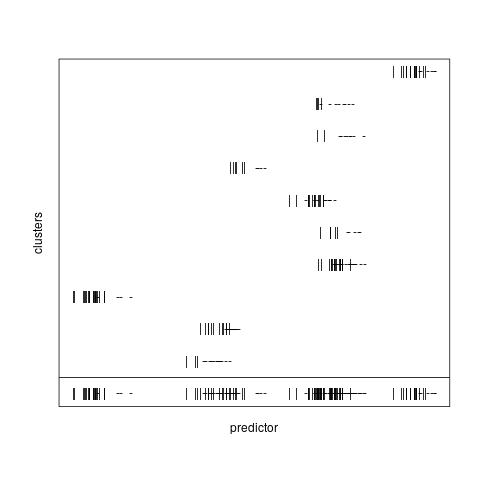
\includegraphics[width=0.5\textwidth]{211223a.png}}
  \hfill
  \subfloat{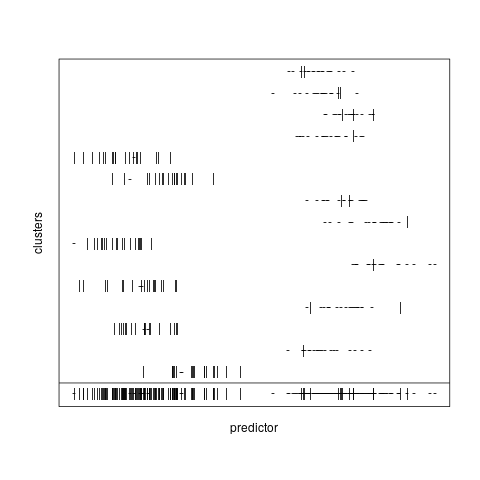
\includegraphics[width=0.5\textwidth]{211223b.png}}
  \caption{Two visualizations contrasting the individual and
    population AUCs. Each plots data from ten clusters sampled IID
    according to a binormal model and at the bottom the unclustered
    population. Case observations are represented with ``$-$'' and
    control observations with ``$|$''. On the left, the individual AUC is
    informative and the population AUC uninformative. The reverse situation is
    presented on the right.}  \label{fig:comparison}
\end{figure}










\subsection{Simplifications when $(X,Y)\cind (M,N)$}

Under some conditions, the cluster AUC parameters $\aucpop$ and
$\aucindiv$ may simplify to the $M=N=1$ case. An example is given in
[[ref section example]], where the exchangeable cluster structure
enables the simplification.
\begin{proposition}\label{proposition:reduction} Given $(X,Y,M,N)\sim \P$, suppose $(X,Y)$ is independent of $(M,N)$ and that $\E\kernel(X_{1k},Y_{1l})$ does not depend on $k,l$. Then $\aucindiv(\P)=\E\kernel(X_{11},Y_{11})$ and $\aucpop(\P)=\E\kernel(X_{11},Y_{21})$.
\end{proposition}

\begin{proof}
  \begin{align}
    \aucindiv(\P) &= \E\left(\frac{\sum_{k=1}^M\sum_{l=1}^N\kernel(X_{1k},Y_{1l})}{MN}\right)\\
                  &=\E\left(\frac{1}{MN}\E\left(\sum_{k=1}^M\sum_{l=1}^N\kernel(X_{1k},Y_{1l}) \mid M,N\right)\right)\\
                  &=\E\left(\frac{1}{MN}MN\E\kernel(X_{11},Y_{11})\right) = \E\kernel(X_{11},Y_{11}).                    
  \end{align}
  Lemma \ref{lemma:conditional wald} was used to get the third equality.

  If $\E\kernel(X_{1k},Y_{1l})$ does not depend on $k,l$, then neither does $\E\kernel(X_{1k},Y_{2l})$. Similar to the above,
  \begin{align}
    \aucpop(\P) &= \frac{\E\left(\sum_{k=1}^{M_1}\sum_{l=1}^{N_2}\kernel(X_{1k},Y_{2l})\right)}{\E(M)\E(N)}\\
    &=\frac{\E(M)\E(N)\E\kernel(X_{11},Y_{21})}{\E(M)\E(N)} = \E\kernel(X_{11},Y_{21}).
  \end{align}
\end{proof}


\begin{lemma}\label{lemma:conditional wald}
  Given random variables $M,V,X_1,X_2,\ldots,$ such that $M\in\{1,2,\ldots\}, \E|M|<\infty ...$ [[other moment conditions]]
  \begin{align}
    \E\left(\sum_{i=1}^M X_i \bigg\vert M,V\right) = \sum_{i=1}^M \E(X_i\mid M,V)
  \end{align}
\end{lemma}
\begin{proof}
  \begin{align}
    \E\left(\sum_{i=1}^M X_i\bigg\vert M,V\right)
    &=  \E\left(\sum_{m=1}^\infty\{M=m\}\sum_{i=1}^m X_i\bigg\vert M,V\right)\\
    &= \sum_{m=1}^\infty \E\left(\{M=m\}\sum_{i=1}^m X_i\bigg\vert M,V\right)\\
    &=\sum_{m=1}^\infty \sum_{i=1}^m\{M=m\}\E(X_i\mid M,V)\\
    &=\sum_{i=1}^M\E(X_i\mid M,V).
    % &=\sum_{i=1}^\infty\{M\ge i\}\E(X_i\mid M,V)
  \end{align}
  [[justify interchange in 2nd equality]]
\end{proof}

[[theorem on bounds]]


In order for $\aucpophat\to 1$ while $\aucindivhat\not\to 1$ in the
random effects model discussed in [[reff section example]], it was
necessary that $(X,Y)\not\cind (M,N)$. Theorem [[ref theorem on
bounds]] bounds $\aucpop$ by $\aucindiv$ under a particular simple
case of $(X,Y)\cind (M,N)$, when $M$ and $N$ are each constant.


We introduce the bound in the simple case. Each cluster contributes
just one control and one case observation each, and their joint
distribution $\P$ is supported on finitely many points in the
plane:  %regarding $\P$ as their joint distribution of $(X,Y)$, let this be a finite sum of atoms in the plane,
\begin{align}
  &\P = \sum_{i=1}^\B p_i \delta_{(x_i,y_i)}\\
  &(x_i,y_i) \in \mathbb{R}^2 \text{ and } 0\le p_i\le 1,i=1,\ldots,B\\
  &p_1+\ldots+p_\B=1.
\end{align}
For this simple example, assume further that all the $x_i$ and $y_i$ are distinct, so in
particular $\psi(x,y)=\{x<y\}$.

The individual AUC is
$$\aucindiv(P)=\P(X<Y)=\underset{i:x_i<y_i}{\sum} p_i.$$
The population AUC depends on the marginal distributions of $X$ and
$Y$, say, $\Pind$,
$$\theta_{12}(\P)=\Pind(X<Y).$$
Since all the $x$-coordinates of the support points are distinct, the
marginal distribution of $X$ is simply
$\Pind(X=x)=\sum_i p_i\delta_{x_i}(x)$. Similarly,
$\Pind(Y=y)=\sum_i p_i\delta_{y_i}(y).$ The product measure is
therefore a sum of $B^2$ atoms,
$\Pind(X=x,Y=y)=\sum_{i,j}p_ip_j\delta_{(x_i,y_j)}(x,y)$. We give a
lower bound for the population AUC $\Pind(X<Y)$. An atom of $\P$ lying
in $\{x<y\}$ of mass $p$ contributes $p_i^2$ to the mass of
$\Pind(X<Y)$. Each pair of atoms of $\P$ lying in $\{x<y\}$ of mass
$p$ and $q$ contributes at least $pq$ and possibly $2pq$ to the mass
of $\Pind(X<Y)$. See Fig. [[ref]].% For, if $x_i<x_j$ then $x_i<y_j$ and
% $(x_i,y_j)\in\{x<y\}$, while if $x_i>x_j$ then
% $(x_j,y_i)\in\{x<y\}$. See Fig. [[ref]]. Either way a contribution of
% at least $p_ip_j$ to the mass of $\{x<y\}$ under
% $\P_{\cind}$. 
Therefore
\begin{align}
  \aucpop(\P)&=\Pind(X<Y) \ge \sum_{i:x_i<y_i} p_i^2 +
           \sum_{i:x_i<y_i}\underset{\substack{j:x_j<y_j\\i<j}}{\sum} p_ip_j\\
         &= \frac{1}{2}\left(\underset{i:x_i<y_i}{\sum} p_i\right)^2 +
           \frac{1}{2}\underset{i:x_i<y_i}{\sum} p_i^2\\
         &\ge \frac{1}{2}\left(\underset{i:x_i<y_i}{\sum} p_i\right)^2 +
           \frac{1}{2|\{i:x_i<y_i\}|}\left(\underset{i:x_i<y_i}{\sum} p_i\right)^2\\
         &= \frac{1}{2}(1+|\{i:x_i<y_i\}|^{-1})\P(X<Y)^2\\
         &= \frac{1}{2}(1+|\{i:x_i<y_i\}|^{-1})\aucindiv(\P)^2.\\
\end{align}
The first inequality is tight when each each pair $i,j$ such that
$x_i<y_i$ and $x_j<y_j$ contributes exactly $p_ip_j$, i.e., when the
square given by $x_i,x_j$ and $y_i,y_j$ has exactly one corner in
$\{x<y\}$. See Fig. [[ref]]. Assuming $x_i<x_j$, this occurs when
$y_i-x_i < x_j-x_i$.  The second inequality is Cauchy-Schwarz, and is
tight when all the atoms in $\{x<y\}$ have the same mass.

By symmetry,
$$
\P_{\cind}(X>Y) \ge \frac{1}{2}(1+|\{i:x_i>y_i\}|^{-1})\P(X>Y)^2,
$$
leading to an upper bound
% \begin{align}
%   \aucpop &= \P_{\cind}(X<Y) = 1 - \P_{\cind}(X>Y)\\
%           &\le 1 - \frac{1}{2}(1+|\{i:x_i>y_i\}|^{-1})\P(X>Y)^2\\
%           &= 1 - \frac{1}{2}(1+|\{i:x_i>y_i\}|^{-1})(1-\aucindiv)^2.
% \end{align}
\begin{align}
  \aucpop \le 1 - \frac{1}{2}(1+|\{i:x_i>y_i\}|^{-1})(1-\aucindiv)^2.
\end{align}
Simplifying and combining these bounds,
\begin{align}
  \frac{1}{2}\aucindiv^2 \le \aucpop \le 1 - \frac{1}{2}(1-\aucindiv)^2,\\
\end{align}
or equivalently,
\begin{align}
  1-\sqrt{2(1-\aucpop)} \le \aucindiv \le \sqrt{2\aucpop}.
\end{align}
When the individual AUC is completely uninformative, $\aucindiv=1/2$,
the informativity of the population AUC is limited,
$1/8 \le \aucpop \le 7/8$. However, when the population AUC is
completely uninformative, $\aucpop=1/2$, the above bounds on the individual AUC, which are tight, are vacuous, $0\le\aucindiv\le 1$. Situations as described in Section [[ref]], where the population AUC $\to 1$ while the individual AUC $\to 1/2$, appears to require some dependence between $M,N$ and $X,Y$. % Though we do not completely prove this below, giving the bounds not for any $(M,N)\cind (X,Y)$ but specifically for constant $M,N$.


\begin{figure}[!tbp]
  \centering
  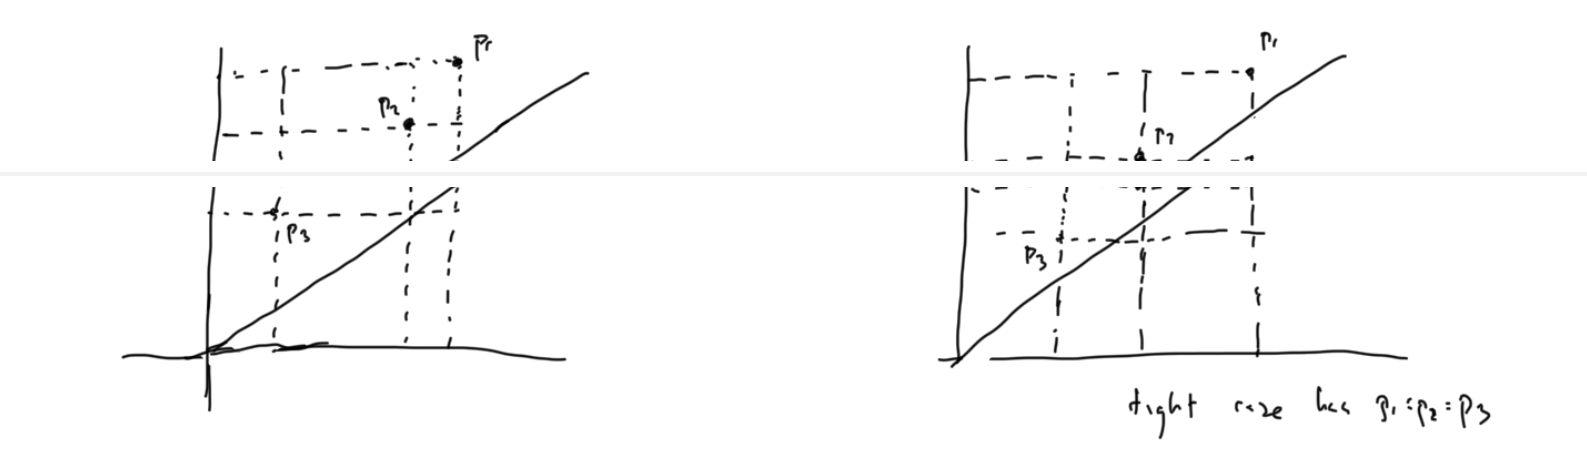
\includegraphics[width=\textwidth]{220103.png}
  \caption{The case $M=N=1$ and finitely supported $(X,Y)$. When the
    distance between the atoms $p_1$ and $p_2$ is small
    relative to their distances to the line $x=y$, they contribute
    $p_1p_2$ to the product of the marginals. When it is relatively
    large, they contribute $2p_1p_2$.}  \label{fig:inequality}
\end{figure}


Theorem \ref{theorem:bounds} extends the inequality to an arbitrary probability measure on the plane $\P$ so long as $M$ and $N$ are constant.

\begin{theorem}\label{theorem:bounds}
  Let $(X,Y,M,N)\sim \P$ be given as in [[ref background]]. Assume
  further that $M=m$ and $N=n$ are constant. Then
  \begin{align}
    \frac{1}{2}\left(\aucindiv+\frac{\sum_{k,l}\P(X_{1k}=Y_{1l})}{2mn}\right)^2 \le \aucpop \le 1-\frac{1}{2}\left(1-\aucindiv+\frac{\sum_{k,l}\P(X_{1k}=Y_{1l})}{2mn}\right)^2
  \end{align}
  % [[drop 1 and 2 from X/Y observations in favor of primes throughout?]]
\end{theorem}
% Lemma for ($m=n=1$ case).
\begin{lemma}\label{lemma:bounds}  Given a pair of scalar random variables $(X,Y)$ with joint distribution $\P$, let $\P_{\cind}$ be the product measure of the marginals, i.e., for all real $a,b$,
  $$
  \P_{\cind}(\{x<a\}\cap\{y<b\})=\P(\{x<a\})\P(\{y<b\}).
  $$
  Then
  \begin{align}
    \frac{1}{2}(\P(X<Y)+\P(X=Y))^2 \le \P_{\cind}(X<Y)+\frac{1}{2}(X=Y)
    \le 1-\frac{1}{2}(1-\P(X<Y))^2.
  \end{align}
\end{lemma}

With the random vector $(X,Y,M,N) \sim \P$, with constant $M=N=1$ and so $\P$ may be regarded as the joint distribution of $(X,Y)$, the conclusion of the Lemma is
\begin{align}
  \frac{1}{2}(\aucindiv(\P)+\frac{1}{2}\P(X=Y))^2 \le \aucpop(P)
  \le 1-\frac{1}{2}(1-\aucindiv(\P)+\frac{1}{2}\P(X=Y))^2.
\end{align}

\begin{proof}[Proof of Lemma \ref{lemma:bounds}]
  Define for $n\in\mathbbm{N}$ approximations to $\aucindiv$ and $\aucpop$ by
  \begin{align}
    A_{ij}^{(n)} &= \left\{(x,y) : \frac{i}{2^n}\le x<\frac{i+1}{2^n},
    \frac{j}{2^n}\le y<\frac{j+1}{2^n}\right\},
    \hspace{.1in}-2^{2n}\le i,j < 2^{2n}-1\\
    \aucindiv^{(n)} &= \sum_{i=-2^{2n}}^{2^{2n}-1}\sum_{j=i+1}^{2^{2n}-1} \P(A_{ij}^{(n)})
                      + \frac{1}{2}\sum_{i=-2^{2n}}^{2^{2n}-1} \P(A_{ii}^{(n)})\\
    \aucpop^{(n)} &= \sum_{i=-2^{2n}}^{2^{2n}-1}\sum_{j=i+1}^{2^{2n}-1} \Pind(A_{ij}^{(n)})
                    + \frac{1}{2}\sum_{i=-2^{2n}}^{2^{2n}-1} \Pind(A_{ii}^{(n)}).
  \end{align}
  % and analogously for an approximation $\aucpop^{(n)}$ to $\aucpop$ using the product of the marginals $\Pind$ rather than $\P$
%   \begin{align}
% ,
%   \end{align}
  Since $\bigcup_n \bigcup_i\bigcup_{j>i} A_{ij}^{(n)} = \{x < y\}$ and 
    $\bigcap_n\bigcup_i A_{ii}^{(n)} = \{x=y\},$
  % \begin{align}
    % \bigcup_n \bigcup_i\bigcup_j A_{ij}^{(n)} &= \{x < y\}\\
    % \bigcap_n\bigcup_i A_ii^{(n)} &= \{x=y\}
  % \end{align}
    by continuity of measure $\aucindiv^{(n)}\to\aucindiv$ and $\aucpop^{(n)}\to\aucpop$. Therefore, it is enough to establish the inequality [[ref theorem conclusion display]] for $\aucindiv^{(n)}$ and $\aucpop^{(n)}$.

    Fix $n$
    \begin{align}
      &\sum_{i=-2^{2n}}^{2^{2n}-2}\sum_{j=i+1}^{2^{2n}-1} \Pind(A_{ij}^{(n)})
      = \sum_{i=-2^{2n}}^{2^{2n}-2}\sum_{j=i+1}^{2^{2n}-1} \Pind(A_{ij}^{(n)})\\
      &= \sum_{i=-2^{2n}}^{2^{2n}-2}\sum_{j=i+1}^{2^{2n}-1} \Pind(\frac{i}{2^n}\le x<\frac{i+1}{2^n})
        \Pind(\frac{j}{2^n}\le y<\frac{j+1}{2^n})\\
      &\ge \sum_{i=-2^{2n}}^{2^{2n}-2}\sum_{j=i+1}^{2^{2n}-1}
        (\A{ii}+\sum_{k=i+1}^{2^{2n}-1}\A{ik})
        (\A{jj}+\sum_{l=-2^{2n}}^{j-1}\A{lj})\\
      &= \sum_{i=-2^{2n}}^{2^{2n}-2}\sum_{j=i+1}^{2^{2n}-1}\left(
        \sum_{k=i+1}^{2^{2n}-1}\A{ik}\sum_{l=-2^{2n}}^{j-1}\A{lj} +
        \A{ii}\sum_{l=-2^{2n}}^{j-1}\A{lj} +
      \A{jj}\sum_{k=i+1}^{2^{2n}-1}\A{ik} +
        \A{ii}\A{jj}
    \right).
    \end{align}
    Handle in turn the first three terms in parentheses.

    First term:
    \begin{align}
     &      \sum_{i=-2^{2n}}^{2^{2n}-2}\sum_{j=i+1}^{2^{2n}-1}
      \sum_{k=i+1}^{2^{2n}-1}\A{ik}\sum_{l=-2^{2n}}^{j-1}\A{lj}\\
      &=            \sum_{i=-2^{2n}}^{2^{2n}-2}\sum_{k=i+1}^{2^{2n}-1}\A{ik}
        \sum_{j=i+1}^{2^{2n}-1}
      \sum_{l=-2^{2n}}^{j-1}\A{lj}\\
      &\ge            \sum_{i=-2^{2n}}^{2^{2n}-2}\sum_{k=i+1}^{2^{2n}-1}\A{ik}
        \sum_{j=i+1}^{2^{2n}-1}
      \sum_{l=i}^{j-1}\A{lj}\\
      &=            \sum_{i=-2^{2n}}^{2^{2n}-2}\sum_{k=i+1}^{2^{2n}-1}\A{ik}
        \sum_{l=i}^{2^{2n}-2} \sum_{j=l+1}^{2^{2n}-1}   \A{lj}\\
      &=            \sum_{i=-2^{2n}}^{2^{2n}-2}\sum_{k=i+1}^{2^{2n}-1}\A{ik}
         \sum_{j=i+1}^{2^{2n}-1} \A{ij} +
        \sum_{i=-2^{2n}}^{2^{2n}-2}\sum_{k=i+1}^{2^{2n}-1}\A{ik}
        \sum_{l=i+1}^{2^{2n}-2} \sum_{j=l+1}^{2^{2n}-1} \A{lj}\\
      &\ge \sum_{i=-2^{2n}}^{2^{2n}-2}\sum_{j=i+1}^{2^{2n}-1}\A{ij}^2 +
        \sum_{i=-2^{2n}}^{2^{2n}-2}\sum_{k=i+1}^{2^{2n}-2}
        \sum_{j=k+1}^{2^{2n}-1} \A{ij} \A{ik} +
                \sum_{i=-2^{2n}}^{2^{2n}-2}\sum_{k=i+1}^{2^{2n}-1}\A{ik}
        \sum_{l=i+1}^{2^{2n}-2} \sum_{j=l+1}^{2^{2n}-1} \A{lj}\\
      &= \underset{\substack{i\neq k \text{ or } j\neq l\\j>i\text{ and }l>k}}
      {\sum\sum\sum\sum}\A{ij}\A{kl} + \sum_{i=-2^{2n}}^{2^{2n}-2}\sum_{j=i+1}^{2^{2n}-1}\A{ij}^2 \\
      &= \frac{1}{2}\left(\sum_{i=-2^{2n}}^{2^{2n}-2}\sum_{j=i+1}^{2^{2n}-1}\A{ij}\right)^2 +
         \frac{1}{2}\sum_{i=-2^{2n}}^{2^{2n}-2}\sum_{j=i+1}^{2^{2n}-1}\A{ij}^2 .
    \end{align}


    Middle two terms:

    \begin{align}
            & \sum_{i=-2^{2n}}^{2^{2n}-2}\sum_{j=i+1}^{2^{2n}-1}\left(
        \A{ii}\sum_{l=-2^{2n}}^{j-1}\A{lj} +
              \A{jj}\sum_{k=i+1}^{2^{2n}-1}\A{ik} \right)\\
      &= \sum_{i=-2^{2n}}^{2^{2n}-2}\A{ii}\sum_{l=i}^{2^{2n}-2}
        \sum_{j=l+1}^{2^{2n}-1}\A{lj} +
        \sum_{j=-2^{2n}+1}^{2^{2n}-1}\A{jj}\sum_{i=-2^{2n}}^{j-1}
        \sum_{k=i+1}^{2^{2n}-1}\A{ik}\\
      &= \sum_{i=-2^{2n}}^{2^{2n}-2}\A{ii}\sum_{l=i}^{2^{2n}-2}
        \sum_{j=l+1}^{2^{2n}-1}\A{lj} +
        \sum_{i=-2^{2n}+1}^{2^{2n}-1}\A{ii}\sum_{l=-2^{2n}}^{i-1}
        \sum_{j=l+1}^{2^{2n}-1}\A{lj}\\
            &=\left(\sum_{i=-2^{2n}}^{2^{2n}-1}\A{ii}\right)
              \left(\sum_{l=-2^{2n}}^{2^{2n}-2}\sum_{j=l+1}^{2^{2n}-1}\A{lj}\right).
    \end{align}
    Second to last equality is just renaming indices.
    
    % The final term is

    % \begin{align}
    %   & \sum_{i=-2^{2n}}^{2^{2n}-2}\sum_{j=i+1}^{2^{2n}-1} \A{ii}\A{jj}
    %   =
          %       \end{align}

    With these lower bounds,
    \begin{align}
    \aucpop^{(n)} &= \sum_{i=-2^{2n}}^{2^{2n}-1}\sum_{j=i+1}^{2^{2n}-1} \Pind(A_{ij}^{(n)})
                    + \frac{1}{2}\sum_{i=-2^{2n}}^{2^{2n}-1} \Pind(A_{ii}^{(n)})\\
                  &\ge \frac{1}{2}\left(\sum_{i=-2^{2n}}^{2^{2n}-2}\sum_{j=i+1}^{2^{2n}-1}\A{ij}\right)^2 +
                    \left(\sum_{i=-2^{2n}}^{2^{2n}-1}\A{ii}\right)
                    \left(\sum_{l=-2^{2n}}^{2^{2n}-2}\sum_{j=l+1}^{2^{2n}-1}\A{lj}\right) +\\
                  &\sum_{i=-2^{2n}}^{2^{2n}-2}\sum_{j=i+1}^{2^{2n}-1} \A{ii}\A{jj}
                    + \frac{1}{2}\sum_{i=-2^{2n}}^{2^{2n}-1} \P(A_{ii}^{(n)})^2\\
                  &= \frac{1}{2}\left(\sum_{i=-2^{2n}}^{2^{2n}-2}\sum_{j=i+1}^{2^{2n}-1}\A{ij} +
                    \sum_{i=-2^{2n}}^{2^{2n}-1} \P(A_{ii}^{(n)})\right)^2\\
      &= \frac{1}{2}\left(\aucindiv^{(n)} +\frac{1}{2}\sum_{i=-2^{2n}}^{2^{2n}-1} \P(A_{ii}^{(n)})\right)^2.\\
      &= \frac{1}{2}\left(\aucindiv^{(n)} +\frac{1}{2}\P(X=Y)\right)^2+o(1).\\
    \end{align}
     The upper bound then follows by the same symmetry argument as given in Section [[ref section m=n=1 case]]
    
  \end{proof}

\begin{proof}[Proof of Theorem \ref{theorem:bounds}]

  % ($m\ge 1, n\ge 1$)
  With
  $$
  \aucindiv = \frac{1}{mn}\E(\Kernel_{11}) = \frac{1}{mn}\sum_{i,j}(\P(X_{1i}<Y_{1j})+\frac{1}{2}\P(X_{1i}=Y_{1j}))
  $$
  Lemma \ref{lemma:bounds} gives
  \begin{align}
    \aucpop &= \frac{1}{mn}\E(\Kernel_{12}) = \frac{1}{mn}\sum_{i,j}(P(X_{1i}<Y_{2j})+\frac{1}{2}\P(X_{1i}=Y_{2j}))\\
    &\ge \frac{1}{mn}\sum_{i,j}\frac{1}{2}(\P(X_{1i}<Y_{1j})+\P(X_{1i}=Y_{1j}))^2
  \end{align}
  continuing with Jensen's inequality
  \begin{align}
    &\ge \frac{1}{2}\left(\frac{1}{mn}\sum_{i,j}(\P(X_{1i}<Y_{1j})+\P(X_{1i}=Y_{1j}))\right)^2\\
    &= \frac{1}{2}\left(\aucindiv + \frac{1}{2mn}\sum_{i,j}\P(X_{1i}=Y_{1j})\right)^2.
  \end{align}
  The other bound follows similarly.
  [[maybe switch to $P$ and $\P_\cind$ notation above]]


  Jensen bound achieved with the pairwise AUCs are all equal.
\end{proof}



\subsection{Relation to Simpson's Paradox}
classic simpsons paradox examples: contingency tables, regression

could make connection to contingency tables explicit using confusion
matrix, however, would require going to ROC origins of AUC, otherwise
not needed for the manuscript.









\subsection{Asymptotic Distribution of $(\aucpop,\aucindiv)$}

stated in greater generality than auc setting. as discussed [[ref]]
$(\psi,m,n)$ is a sufficient statistic. let $W=(Z,M,N)\sim
P$. $\Kernel$ is a real-valued function on pairs $(W,W')$ [[domain of
psi since vectors are variable length??]]  define $\aucpop$ and
$\aucindiv$ in terms of suff stat ... as well as estimators ... .

\begin{theorem}\label{theorem:asymptotic} Let $\psi:V\times V\to\mathbb{R}$, $(X,Y,M,N)\sim\P$ with $(X,Y)\in V\times V$, $\psi\in L^2(\P)$, $M$ and $N$ counting numbers $\ge 0$ with finite means. Then
  \begin{align}
    \sqrt{\I}(\aucpophat-\aucpop,\aucindivhat-\aucindiv) \leadsto \mathcal{N}(0,\Sigma)
  \end{align}
  with
  \begin{align}
    \Sigma_{11} &= \lim_{\I\to\infty} \I\V(\aucpophat) =
    \E\left(\frac{\E(\Kernel_{12}\mid\W_1)+\E(\Kernel_{21}\mid\W_1)}{\E M\E N} - \aucpop\left(\frac{M_1}{\E M} + \frac{N_1}{\E N}\right)   \right)^2
    \\
    \Sigma_{22} &= \lim_{\I\to\infty} \I\V(\aucindivhat) =
    \V(\Kernel_{11}/(M_1N_1))
    \\
    \Sigma_{12} &= \lim_{\I\to\infty} \I\cov(\aucpophat,\aucindivhat) =
    \aucpop\E\left(\frac{\Kernel_{11}}{M_1N_1}\left(\frac{\Kernel_{12}+\Kernel_{21}}{\E\Kernel_{12}} - \frac{M_1}{\E M}-\frac{N_1}{\E N}  \right) \right)
  \end{align}
  % $\sqrt{\I}(\aucpophat-\aucpop,\aucindivhat-\aucindiv) $ converges to a mean-zero bivariate normal distribution with covariance matrix given by
  % \begin{align}
  % \end{align}
\end{theorem}


\begin{proof}%[Proof of asy normality]

  By Lemma [[]]
  \begin{align}
    \sqrt{\I}\left(
    \frac{(\I)_2^{-1}\sum_{i\neq j}\Kernel_{ij}-\E\Kernel_{12}}{\sd(\sqrt{\I}(\I)_2^{-1}\sum_{i\neq j}\Kernel_{ij})}
    ,        
    \frac{\I^{-2}\sum_{i,j}M_iN_j - \E M\E N}
    {\sd(\I^{-3/2}\sum_{i, j}M_iN_j ) }
    ,
     \frac{\I^{-1}\sum_i \Kernel_{ii}/(M_iN_i) - \E(\Kernel_{11}/M_1N_1)}
     {\sd(\Kernel_{11}/M_1N_1)}
    \right)
  \end{align}
  converges to
  \begin{align}
    \I^{-1/2}\sum_{i=1}^\I\left(
     \frac{\E(\Kernel_{i0}\mid\W_i)+\E(\Kernel_{0i}\mid\W_i)-2\E\Kernel_{12}}
    {\sd(\E(\Kernel_{10}\mid\W_1)+\E(\Kernel_{01}\mid\W_1))}
    ,
     \frac{M_i\E N + N_i\E M - 2\E M\E N}
     {\sd(M_1\E N + N_1\E M)} 
     ,
     \frac{ \Kernel_{ii}/(M_iN_i) - \E(\Kernel_{11}/M_1N_1)}
    {\sd(\Kernel_{11}/M_1N_1)}
    \right)
  \end{align}
  in mean-square. The latter is an IID sum with finite covariance matrix and is asymptotically normal by the usual CLT.
  % \begin{align}
  % \end{align}
  Applying the delta method with the function
  $(x,y,z)\mapsto (x/y,z)$, with derivative
  $$
  \begin{pmatrix}
    1/y & -x/y^2 & 0 \\
    0 & 0 & 1
  \end{pmatrix}
  $$
  for $y\neq 0$, i.e., $E(M)\neq 0, E(N)\neq 0$, gives the asymptotic normality of $(\aucindiv,\aucpop)$.
  [[asymptotic covariance matrix is given by delta method [[but must track down the 1/2 term--see notes P.3]]

%   \begin{align}
%   \end{align}
%   and by continuity of the delta method function, the same must hold of [[ref target vector]].

  
%   first two components are nearly two sample u-statistics (but dependence across same cluster), last being an average is a 1-sample u-statistic, so we use similar methods. 

  
%   Two steps: Show the asymptotic normality of
%   \begin{align}
%    \sqrt{\I}((I)^{-1}_2\sum_{i,j}\Kernel_{ij} - \E\Kernel_{12}, (\I)^{-2}\sum_{i,j}M_iN_j - \E(MN), \I^{-1}\sum_i \Kernel_{ii}/(M_iN_i)).
%   \end{align}
%   Then apply delta method with the function $(x,y,z)\mapsto (x/y,z)$, with derivative
%   $$
%   \begin{pmatrix}
%     1/y & -x/y^2 & 0 \\
%     0 & 0 & 1
%   \end{pmatrix}
%   $$
%   for $y\neq 0$, i.e., $E(M)\neq 0, E(N)\neq 0$.


%   For first step: Whow asy normality of [[ref above]] by showing each component
%   converges in $L_2$ to an iid sum. Third component is already an iid sum, so only need to take care of the first two components.

% condition on setof sums ....
%   falling factorial notation $(\I)_n=\prod_{i=0}^{n-1}(I-i)$ for $n\ge 1$.

%   first component:

%   The $L_2$ projection of $\E((\I)_2^{-1}\sum_{i\neq j}\Kernel_{ij} - \E\Kernel_{12}$ onto the subspace ... is
%   \begin{align}
%     \I^{-1}\sum_{i=1}^\I(\E(\Kernel_{i0}\mid \W_i) + \E(\Kernel_{0i}\mid\W_i)) -2\E\Kernel_{12}
%   \end{align}
%   and the variance of the projection, multiplied by $\I$, is
%   \begin{align}
%     \V(\E(\Kernel_{12}\mid\W_1) + \E(\Kernel_{21}\mid \W_1)).
%   \end{align}
%   The normalized variance of the first component of [[ref vector]] is
%   \begin{align}
%     \I\V((\I)_2^{-1}\sum_{i\neq j}\Kernel_{ij}) &=
%                                                   \I(\I_2^{-2}(\I)_3(\cov(\Kernel_{12},\Kernel_{13})+\cov(\Kernel_{21},\Kernel_{31}) +2\cov(\Kernel_{12},\Kernel_{31}))\\
%                                                 &= \frac{\I-2}{\I-1}(\E\Kernel_{12}\Kernel_{13}+\E\Kernel_{21}\Kernel_{31}+2\E\Kernel_{12}\Kernel_{31}-4(\E\Kernel_{12})^2)\\
%                                                 &=\frac{\I-2}{\I-1}(\E(\E(\Kernel_{12}\mid\W_1)^2)+\E(\E(\Kernel_{21}\mid\W_1)^2) + 2\E(\E(\Kernel_{12}\mid\W_1)\E(\Kernel_{21}\mid\W_1)) - 4(\E\Kernel_{12})^2)\\
%                                                 &=\frac{\I-2}{\I-1}(\E(\E(\Kernel_{12}\mid\W_1)+\E(\Kernel_{21}\mid\W_1))^2   - 4(\E\Kernel_{12})^2)\\
%     &=\frac{\I-2}{\I-1}    \V(\E(\Kernel_{12}\mid\W_1) + \E(\Kernel_{21}\mid \W_1)).
%   \end{align}
%   The ratio of these two variances tends to 1, so [[maybe cite vdvaart/serfling]]
%   \begin{align}
%     \bigg|\frac{\sqrt{\I}((\I)_2^{-1}\sum_{i\neq j}\Kernel_{ij}-\E\Kernel_{12})}{\sd(\sqrt{\I}(\I)_2^{-1}\sum_{i\neq j}\Kernel_{ij})}
%     - \frac{\sqrt{\I}(\I^{-1}\sum_{i=1}^\I(\E(\Kernel_{i0}\mid\W_i)+\E(\Kernel_{0i}\mid\W_i)-2\E\Kernel_{12})}
%     {\sd(\I^{-1/2}\sum_{i=1}^\I(\E(\Kernel_{i0}\mid\W_i)+\E(\Kernel_{0i}\mid\W_i)))}\bigg| \underset{L_2}{\to} 0.
%   \end{align}
  
%   second component:

%   The $L_2$ projection of $(\I)^{-1}_2\sum_{i\neq j}M_iN_j-\E(M)\E(N)$ onto the subspace ... is
%   \begin{align}
%     \I^{-1}\sum_{i=1}^\I(M_i\E(N)+N_i\E(M))-2\E(M)\E(N)
%   \end{align}
%   and the variance of the projection, multiplied by $\I$, is
%   \begin{align}
%     &\V(M_1\E(N)+N_1\E(M))\\
%     &=(\E N)^2(\E(M^2)-(\E M)^2) + (\E M)^2(\E(N^2)-(\E N)^2) + 2\E M\E N(\E(MN)-\E M\E N)\\
%     &= \E(M_1\E N + N_2\E M)^2 - 4(\E M\E N)^2.
%   \end{align}
%   The normalized variance of the second component of [[ref vector]] is
%   \begin{align}
%     \I\V((\I)^{-1}_2\sum_{i\neq j}M_iN_j) &=\frac{1}{\I(\I-1)^2}\V(\sum_{i\neq j}M_iN_j)\\
%                                             &=\frac{1}{\I(\I-1)^2}(O(\I^{-2}) + (\I)_3(\cov(M_1N_2,M_1N_3)+\cov(M_2N_1,M_3N_1)+2\cov(M_1N_2,M_3N_1)))\\
%     &\underset{\I\to\infty}{\to} \E(M_1\E N + N_1\E M)^2 - 4(\E M\E N)^2,
%   \end{align}
%   so the ratio of these two variances tends to $1$, and so
%   \begin{align}
%     \bigg|\frac{\sqrt{\I}((\I)_2^{-1}\sum_{i\neq j}M_iN_j - \E M\E N)}
%     {\sd(\sqrt{\I}(\I)_2^{-1}\sum_{i\neq j}M_iN_j ) }
%     - \frac{\sqrt{\I}(\I^{-1}\sum_i(M_i\E N + N_i\E M) - 2\E M\E N)}
%     {\sd(\I^{-1/2}\sum_i(M_i\E N + N_i\E M))} \bigg|
%     \underset{L_2}{\to} 0.
%   \end{align}

%   Next,
%   \begin{align}
%     &|\sqrt{\I}(\I^{-2}\sum_{i,j}M_iN_j - (\I)^{-1}_2\sum_{i\neq j}M_iN_j)|_{L_2}\\
%     &=\I\cdot\E\left( \frac{1}{(\I^2(\I-1))^2}\sum_{i\neq j,k\neq l}M_iN_jM_kN_l
%       + \frac{1}{\I^4}\sum_{i,j}M_iN_iM_jN_j - \frac{2}{\I^4(\I-1)}\sum_{i,j,k : i\neq j}M_iN_jM_kN_k \right)^2\\
%     &=\frac{\I}{(\I^2(\I-1))^2}\left(  (\I)_4(\E M\E N)^2 + O(\I^3)  \right)
%       + \frac{1}{\I^3}((\I)_2(\E(MN))^2 + O(\I))
%       -\frac{2}{\I^3(\I-1)}((\I)_3\E M\E N\E(MN) + O(\I^2)) \\
%     &\to 0.
%   \end{align}
%   This convergence implies
%       \begin{align}
%     \bigg|\frac{\sqrt{\I}(\I^{-2}\sum_{i,j}M_iN_j - \E M\E N)}
%     {\sd(\I^{-3/2}\sum_{i, j}M_iN_j ) }
%     - \frac{\sqrt{\I}((\I)_2^{-1}\sum_{i\neq j}M_iN_j - \E M\E N)}
%     {\sd(\sqrt{\I}(\I)_2^{-1}\sum_{i\neq j}M_iN_j ) } \bigg|
%     \underset{L_2}{\to} 0
%       \end{align}
%       which combined with [[first part of triangle inequality]] implies
%       \begin{align}
%     \bigg|\frac{\sqrt{\I}(\I^{-2}\sum_{i,j}M_iN_j - \E M\E N)}
%     {\sd(\I^{-3/2}\sum_{i, j}M_iN_j ) }
%     - \frac{\sqrt{\I}(\I^{-1}\sum_i(M_i\E N + N_i\E M) - 2\E M\E N)}
%     {\sd(\I^{-1/2}\sum_i(M_i\E N + N_i\E M))} \bigg|
%     \underset{L_2}{\to} 0.
%       \end{align}
  
%   Combining [[ref result for first component and result for second component]]
%   \begin{align}
%     \sqrt{\I}\begin{pmatrix}
%     \frac{(\I)_2^{-1}\sum_{i\neq j}\Kernel_{ij}-\E\Kernel_{12}}{\sd(\sqrt{\I}(\I)_2^{-1}\sum_{i\neq j}\Kernel_{ij})}\\
%     % ,        
%     \frac{\I^{-2}\sum_{i,j}M_iN_j - \E M\E N}
%     {\sd(\I^{-3/2}\sum_{i, j}M_iN_j ) }\\
%     %,
%      \frac{\I^{-1}\sum_i \Kernel_{ii}/(M_iN_i) - \E(\Kernel_{11}/M_1N_1)}
%      {\sd(\Kernel_{11}/M_1N_1)}
%   \end{pmatrix}
%     -%\\
%     \I^{-1/2}\sum_{i=1}^\I\begin{pmatrix}
%      \frac{\E(\Kernel_{i0}\mid\W_i)+\E(\Kernel_{0i}\mid\W_i)-2\E\Kernel_{12}}
%     {\sd(\E(\Kernel_{10}\mid\W_1)+\E(\Kernel_{01}\mid\W_1))}\\
%     % ,
%      \frac{M_i\E N + N_i\E M - 2\E M\E N}
%      {\sd(M_1\E N + N_1\E M)} \\
%      % ,
%      \frac{ \Kernel_{ii}/(M_iN_i) - \E(\Kernel_{11}/M_1N_1)}
%      {\sd(\Kernel_{11}/M_1N_1)}
%   \end{pmatrix}
%     =o_P(1).
%   \end{align}
% The second sequence is asymptotically normal by the CLT, so the first is as well.

\end{proof}




\begin{corollary}
  Under the assumptions of Theorem \ref{theorem:asymptotic}, let
  $(X_1,Y_1,M_1,N_1),\ldots,(X_\I,Y_\I,M_\I,N_\I),$ be IID according
  to $\P$. For $1\le i\le \I$ define
  \begin{align}
    \kernel_{i\cdot}&=\sum_{j=1}^\I \kernel(X_i,Y_j)\\
    \kernel_{\cdot i}&=\sum_{j=1}^\I \kernel(X_j,Y_i)\\
    \phi_i &= \frac{\kernel(X_i,Y_i)}{M_iN_i}.
  \end{align}
  The asymptotic covariance matrix
  $\Sigma$ of $(\aucpophat,\aucindivhat)$ may be consistently
  estimated by $\hat{\Sigma}$ given by
  \begin{align}
    \hat{\Sigma}_{11} &=\frac{1}{\I-1}\sum_{i=1}^\I\left( \frac{\Kernel_{i\cdot}+\Kernel_{\cdot i}}{M_\cdot N_\cdot}-\aucpophat\left(\frac{M_i}{M_\cdot}+\frac{N_i}{N_\cdot}\right) \right)^2\\
    \hat{\Sigma}_{22} &= \frac{1}{\I-1}\sum_{i=1}^\I(\d_i-\d_\cdot)^2\\
    \hat{\Sigma}_{12} &=\frac{1}{\I}\sum_{i=1}^\I\left(\frac{\d_{i}}{\d_{\cdot}}\left(\frac{\Kernel_{i\cdot}+\Kernel_{\cdot i}}{\Kernel_{\cdot\cdot}} - \frac{M_i}{M_\cdot}-\frac{N_i}{N_\cdot}   \right) \right) %\to_p
  \end{align}
\end{corollary}

The estimator $\hat{\Sigma}_{11}$ of the asymptotic variance of $\aucpophat$ is the same as given by [[cite obuchowski]], derived by a different method.

The finite-sample performance of this estimator is examined in Section \ref{section:simulation}.



\section{Simulation}\label{section:simulation}


A popular parametric model for the AUC is the binormal model, so
called since the case and control observations are assumed to follow a
normal distribution [[cite obu, all the old papers]]. Following [[cite
obu]] we extend this model to accommodate clustered data by modeling
the observations as multivariate normal vectors with an exchangeable
correlation structure.
\begin{align}
  (X,Y) \mid (M,N) \sim \mathcal{N}_{M+N}\left(
  \begin{pmatrix}\mu_X\mathbbm{1}_M\\ \mu_Y\mathbbm{1}_N\end{pmatrix},
  \mathbbm{1}_{M+N}\mathbbm{1}_{M+N}^T + (1-\rho)Id_{M+N}
  \right)
\end{align}
That is, the case and control observations of a given cluster all have
unit variance and share the same pairwise correlation $\rho$, $-1/(M+N)\le\rho\le 1$, all the case observations have mean $\mu_Y$ and all the
control observaions mean $\mu_X$. The binormal model is an example of
the random effect model described in [[ref display in example
section]]. As the effect of the random effect is only to change the
intra-cluster correlation or mean, it is actually redundant to the
usual multivariate normal
parameters and omitted from [[ref above display]]. % Moreover, correlations among control observations or among
% case observations within the same cluster do not contribute to the population or
Moreover, further parameters such as for intra-cluster correlations
$\corr(X_{11},X_{12})$, $\corr(Y_{11},Y_{12})$, or for non-unit
variances $\V(X_11)$ and $\V(Y_11)$ [[ check for variances]], are
redundant for modeling AUCs.

Let $\Delta=\mu_Y-\mu_X\ge 0$. Using Proposition \ref{proposition:reduction},
\begin{align}
  \aucpop(P) &= \Phi\left(\frac{\Delta}{\sqrt{2}}\right)\\
  \aucindiv(P) &=  \Phi\left(\frac{\Delta}{\sqrt{2(1-\rho)}}\right)
\end{align}

[[ref auc formulas]] show that $\aucpop$ and $\aucindiv$ are both
$>1/2, 1/2,$ or $<1/2$. We give two benefits. The first is that
$(\aucpop,\aucindiv)$ can be restricted to $[1/2,1]\times[1/2,1]$, and
may then serve as a parameterization of the binormal model [[ref
display]]. Switching the observations designated ``control'' and
``case'' reflects the AUC across $1/2, AUC\mapsto 1-AUC$, so choosing
$\Delta\ge 0$ or restricted an AUC to lie in $[1/2,1]$ rather than
$[0,1/2]$ is not restrictive.[[probably should move this to intro section]]

The second involves testing. Though AUCs are often compared by
magnitude (eg old multi-reader papers), e.g., $H_0:AUC_1-AUC_2>0$, one
is usually interested in the informativity, i.e., $|AUC_1-1/2|$ versus
$|AUC_2-1/2|$. $H_0:AUC_1-AUC_2>0$ indicates that $AUC_1$ is more
informative when both are greater than $1/2$, but less informative if
both are less than $1/2$.  A further complication is that one may be
greater than $1/2$ and the other less, which will not be solved by
switching the roles.[[include the above???]] These complications are
avoided in the binormal model for the individual and population AUCs,
where $>1/2$ or $<1/2$. Thus a test of the order $\aucpop<\aucindiv$
is also a test of informativity $|\aucpop-1/2|<|\aucindiv-1/2|$.

Model for $(M,N)$. The number $M+N$ of combined case and control
observations belonging in a sample is randomly selected from among. To
obtain the allocation to case and control observations, first $M+N$
normal variables are sampled with unit variance and common pairwise
correlation $...= ...$. Then the number $M$ of control observations is
taken to be those greater than $0$, and the remainder the number $N$
of case observations. The greater the correlation, the greater the
imbalance between case and control observations.

\subsection{Coverage}

% Given $M$ and $N$, the control and case observations $X$ and $Y$
% were sampled according to [[ref display]].
The intra-cluster correlation was set to $...$, while $\Delta$ and
$\rho$ were set to correspond to population AUC of $...$ and
individual AUCs of $...$. For each setting of $...$, $...$ replicates
of size $I=...$ were sampled and used to form a confidence ellipse for
$(\aucpop,\aucindiv)$. Specifically, estimates ... are obtained as
given in [[ref section 1 and section asymptotic]]. Under $P$,
$$
\bigg\vert\Sigma^{-1/2}\left(\begin{pmatrix}\aucpop\\
\aucindiv\end{pmatrix}-\begin{pmatrix}\aucpophat\\\aucindivhat\end{pmatrix}\right)\bigg\vert^2
$$
has a chi-squared distribution with 2 degrees of freedom, so that if
$q$ is an upper $\alpha$ quantile of this distribution, then
$$
\left\{\begin{pmatrix}x\\y\end{pmatrix}:\bigg\vert\Sigma^{-1/2}\left(\begin{pmatrix}x\\y\end{pmatrix}-\begin{pmatrix}\aucpophat\\\aucindivhat\end{pmatrix}\right)\bigg\vert^2
< q\right\}
$$
is a level $1-\alpha$ confidence region for $(\aucpop,\aucindiv)$. The
region covers $(\aucpop,\aucindiv)$ iff [[ref display above]] is $<q$.
This process was repeated $...$ times. Results are presented in Table
\ref{table:1}.

\begin{table}
  \begin{tabular}{rrrrrrrrrr}
  \hline
 & theta.12 & theta.11 & D.corr & coverage & bias.theta.11 & bias.theta.12 & vcov.11 & vcov.12 & vcov.22 \\ 
  \hline
1 & 0.60 & 0.60 & 0.00 & 0.90 & 0.01 & 0.00 & -0.04 & -0.03 & -0.02 \\ 
  2 & 0.60 & 0.60 & 0.40 & 0.97 & 0.00 & 0.00 & -0.01 & 0.00 & 0.00 \\ 
  3 & 0.60 & 0.60 & 0.80 & 0.93 & -0.00 & -0.00 & 0.03 & 0.01 & 0.01 \\ 
  4 & 0.60 & 0.60 & 0.95 & 0.90 & -0.01 & 0.00 & -0.05 & -0.02 & -0.01 \\ 
  1.1 & 0.60 & 0.77 & 0.00 & 0.97 & -0.00 & -0.00 & 0.01 & -0.00 & 0.00 \\ 
  2.1 & 0.60 & 0.77 & 0.40 & 1.00 & 0.00 & 0.00 & 0.00 & 0.00 & 0.03 \\ 
  3.1 & 0.60 & 0.77 & 0.80 & 0.97 & 0.00 & -0.00 & 0.01 & -0.00 & 0.05 \\ 
  4.1 & 0.60 & 0.77 & 0.95 & 0.90 & 0.01 & 0.01 & -0.01 & -0.02 & -0.02 \\ 
  1.2 & 0.60 & 0.95 & 0.00 & 1.00 & 0.00 & -0.00 & 0.00 & 0.00 & -0.00 \\ 
  2.2 & 0.60 & 0.95 & 0.40 & 0.87 & 0.00 & 0.00 & -0.00 & -0.00 & -0.03 \\ 
  3.2 & 0.60 & 0.95 & 0.80 & 1.00 & 0.00 & 0.00 & 0.00 & 0.00 & -0.01 \\ 
  4.2 & 0.60 & 0.95 & 0.95 & 0.97 & -0.00 & 0.01 & 0.00 & -0.01 & -0.01 \\ 
  1.3 & 0.80 & 0.80 & 0.00 & 0.90 & 0.00 & 0.00 & 0.00 & 0.00 & -0.00 \\ 
  2.3 & 0.80 & 0.80 & 0.40 & 0.93 & -0.00 & 0.00 & 0.01 & -0.00 & -0.00 \\ 
  3.3 & 0.80 & 0.80 & 0.80 & 0.90 & 0.00 & 0.00 & -0.01 & -0.00 & 0.00 \\ 
  4.3 & 0.80 & 0.80 & 0.95 & 0.93 & -0.00 & 0.00 & -0.02 & 0.00 & 0.00 \\ 
  1.4 & 0.80 & 0.88 & 0.00 & 0.97 & -0.00 & 0.00 & 0.00 & 0.00 & 0.01 \\ 
  2.4 & 0.80 & 0.88 & 0.40 & 0.93 & -0.00 & 0.01 & 0.00 & 0.00 & 0.00 \\ 
  3.4 & 0.80 & 0.88 & 0.80 & 0.87 & 0.01 & 0.01 & 0.01 & 0.01 & -0.01 \\ 
  4.4 & 0.80 & 0.88 & 0.95 & 0.90 & 0.01 & 0.01 & 0.01 & 0.01 & 0.00 \\ 
  1.5 & 0.80 & 0.95 & 0.00 & 0.93 & 0.00 & 0.00 & 0.00 & 0.00 & 0.01 \\ 
  2.5 & 0.80 & 0.95 & 0.40 & 1.00 & -0.00 & -0.00 & 0.00 & -0.00 & 0.02 \\ 
  3.5 & 0.80 & 0.95 & 0.80 & 0.90 & -0.00 & -0.00 & 0.00 & 0.01 & 0.00 \\ 
  4.5 & 0.80 & 0.95 & 0.95 & 1.00 & -0.00 & -0.00 & 0.00 & -0.00 & 0.01 \\ 
   \hline
\end{tabular}

  \caption{coverage simulation}
  \label{table:1}
\end{table}

similar simulation performed with truncated normal.

check D.corr imbalance affects precision as in obuchowski. 

twofold: check the performance of the variance estimator. show that in
the obuchowski study, large difference in the pop auc hwich was
studied and hte indiv auc.

The settings were chosen differences from obu sim: cluster size larger
(should not affect asymptotics, and need to enforce minimum size);


\subsection{Power}

We examine the power of testing the null hypothesis
$H_0:\aucpop=\aucindiv$ using the proposed variance estimators. The
data is generated under the bnormal model [[ref]] using
(aucpop,aucindiv) selected in the unit square. Estimates
$\aucpophat,\aucindivhat,\hat\Sigma$ are obtained. The test is then
carried out by testing the z-statistic
$$
(\aucpophat-\aucindivhat) /
\sqrt{\begin{pmatrix}1&-1\end{pmatrix}^T\hat\Sigma\begin{pmatrix}1\\-1\end{pmatrix}}
$$
for significance.

When $\rho>0$ in [[ref
binormal model display]], the alternatives to $H_0:\aucpop=\aucindiv$
the set $H_A:|\aucpop-1/2|<|\aucindiv-1/2|$, where the individual AUC
is more ifnormative than the population AUC.


The results of the simulation are presented visually in Fig.\ref{fig:power}. [[some summary of results maybe.]]

\begin{figure}
  \centering
  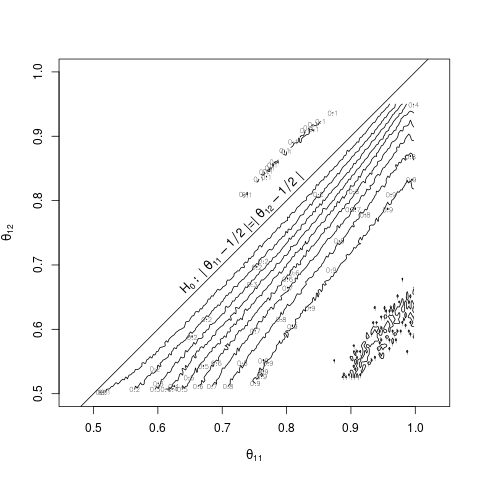
\includegraphics{../sim/211120/211120.png}
  \caption{[[put null in usual format,get rid of artifacts]]}  \label{fig:power}
\end{figure}



difference in magnitude of ind and pop versus difference in
informativity. same for this example.

give power surfaces.

should have table besides figure.
should have something with (m,n) confounding. maybe geenral setting?

\section{Data analysis}

\section{Discussion/Conclusion}
multiple markers

longitudinal analysis

covariates. effectively m,n are the only covariates being considered here.

\bibliographystyle{plain}
\bibliography{auc.bib}


\end{document}

possible additions:
1. conditions (eg location scale) that both theta12 and theta11 are $>1/2$ or $<1/2$ simultaneously. at least can't have delta depend on M,N.
\message{ !name(manuscript.tex) !offset(-1179) }
